\section{Pipeline de Voxelización} % (fold)
\label{sec:pipeline_de_voxelizacion}
El algoritmo de voxelización de escenas es implementado en la clase \emph{VoxelizerRenderer}. Como se explicó en la sección anterior esta es una clase que hereda de la clase Renderer. En el método Render, residen la lógica de voxelización, sombreado de vóxeles, mipmapping para vóxeles anisótropos e iluminación global de vóxeles. En esta sección se describe en detalle solo el proceso de voxelización y su arquitectura.

\subsection{Voxelización Conservativa} % (fold)
\label{sub:voxelization_impl}
Nuestra implementación utiliza una representación simplificada de la escena en vóxeles, esta representación es generada de forma conservativa por tanto si existe algún triangulo dentro del espacio de un vóxel se generara un vóxel por más pequeño que sea este triángulo.
 
\subsubsection{Matrices de Proyección por Eje}

Como se explicó en la sección \ref{sub:voxelizacion_conservativa} cada triangulo debe ser proyectado sobre un eje direccional. El primer paso a realizar es definir estas matrices de proyección. Estas están definidas por una \ac{AABB}. En nuestra implementación se toma la \ac{AABB} que envuelve toda la escena por simplicidad. En el código \ref{UpdateProjectionMatrices} se encuentra el algoritmo de la función que realiza esto. Esta método es llamada cada vez que se cambia carga una escena o cuando se cambiar la resolución de la representación en vóxeles.

La \ac{AABB} puede estar definida de dos formas: por un punto que indica el centro de la caja y un vector extensión que indica la longitud media de la caja en cada eje a partir del centro o por un punto mínimo y un punto máximo. 

En el código se observa que primero se obtiene la longitud total en cada eje que define la \ac{AABB} que envuelve la escena. Luego en la misma función se actualizan dos variables: \emph{volumeGridSize} que indica el tamaño de la cuadricula tridimensional de vóxeles en espacio de mundo y \emph{voxelSize} que indica el tamaño de cada vóxel dentro de esta cuadricula. 

El tronco de proyección es un cubo uniforme por tanto se utiliza la mayor longitud según cada eje. Esto asegura que desde cualquier eje direccional la proyección abarca toda la escena. De esta longitud se extrae la matriz de proyección ortogonal. Luego se configura cada matriz de vista por cada eje direccional. Finalmente se almacena la multiplicación de ambas matrices.
\\
\begin{lstlisting}[caption={Creación de matrices de proyección ortogonal por cada eje direccional}, label=UpdateProjectionMatrices]
void VoxelizerRenderer::UpdateProjectionMatrices(const BoundingBox &sceneBox)
{
    auto axisSize = sceneBox.Extent() * 2.0f;
    auto &center = sceneBox.Center();
    volumeGridSize = glm::max(axisSize.x, glm::max(axisSize.y, axisSize.z));
    voxelSize = volumeGridSize / volumeDimension;
    auto halfSize = volumeGridSize / 2.0f;
    // projection matrices
    auto projection = glm::ortho(-halfSize, halfSize, -halfSize, halfSize, 0.0f, volumeGridSize);
    // view matrices
    viewProjectionMatrix[0] = lookAt(center + glm::vec3(halfSize, 0.0f, 0.0f), center, glm::vec3(0.0f, 1.0f, 0.0f));
    viewProjectionMatrix[1] = lookAt(center + glm::vec3(0.0f, halfSize, 0.0f), center, glm::vec3(0.0f, 0.0f, -1.0f));
    viewProjectionMatrix[2] = lookAt(center + glm::vec3(0.0f, 0.0f, halfSize), center, glm::vec3(0.0f, 1.0f, 0.0f));
    // multiply projection with view
    for (auto &matrix : viewProjectionMatrix)
    {
        matrix = projection * matrix;
    }
}
\end{lstlisting}

Una vez obtenidas las matrices de proyección el algoritmo procede a voxelizar la escena. El proceso de voxelización estática y dinámica utilizan el mismo programa de sombreado o \emph{shader}, la diferencia reside sobre cual geometría es enviada al pipeline de rasterización y durante el fragment shader si se lee o se escribe sobre una textura que indica las posiciones de vóxeles estáticos.

\subsubsection{Selección del Eje Dominante}
Para maximizar el área de voxelización y generar la mayor cantidad de fragmentos posibles cada triangulo es proyectado sobre uno de los ejes direccionales. Este eje se escoge según la normal definida por el plano formado por los tres vértices del triángulo. Este proceso se realiza en el geometry shader. En el geometry shader se puede realizar operaciones sobre los vértices generales por el procesador de vértices o \emph{vertex shader}. Esto es de particular interés para el proceso de voxelización conservativa ya que como fue explicado anteriormente cada vértice de cada triangulo necesita ser expandido.
\\
\begin{lstlisting}[caption={Selección del eje dominante para la proyección ortogonal.}, label=CalculateAxis]
int CalculateAxis()
{
	vec3 p1 = gl_in[1].gl_Position.xyz - gl_in[0].gl_Position.xyz;
	vec3 p2 = gl_in[2].gl_Position.xyz - gl_in[0].gl_Position.xyz;
	vec3 faceNormal = cross(p1, p2);

	float nDX = abs(faceNormal.x);
	float nDY = abs(faceNormal.y);
	float nDZ = abs(faceNormal.z);

	if( nDX > nDY && nDX > nDZ )
    {
		return 0;
	}
	else if( nDY > nDX && nDY > nDZ  )
    {
	    return 1;
    }
	else
    {
	    return 2;
	}
}
\end{lstlisting}

En el algoritmo \ref{CalculateAxis} primero se obtiene la normal del triángulo. El arreglo \emph{gl\_in} contiene información de todos los vértices generados por el vertex shader. Para la aplicación esto es forzado a solo triángulos, por tanto la longitud de gl\_in siempre es tres. Luego según el peso en cada eje de la normal del plano se escoge un eje direccional. Esto se retorna en forma de un número entero. Este número entero indica cuál de las matrices de proyección generadas en la sección anterior va ser utilizada para proyectar cada vértice del triángulo.

\begin{figure}[H]
	\centering
	\begin{subfigure}[t]{.49\linewidth}
		\centering
		\captionsetup{justification=centering}
		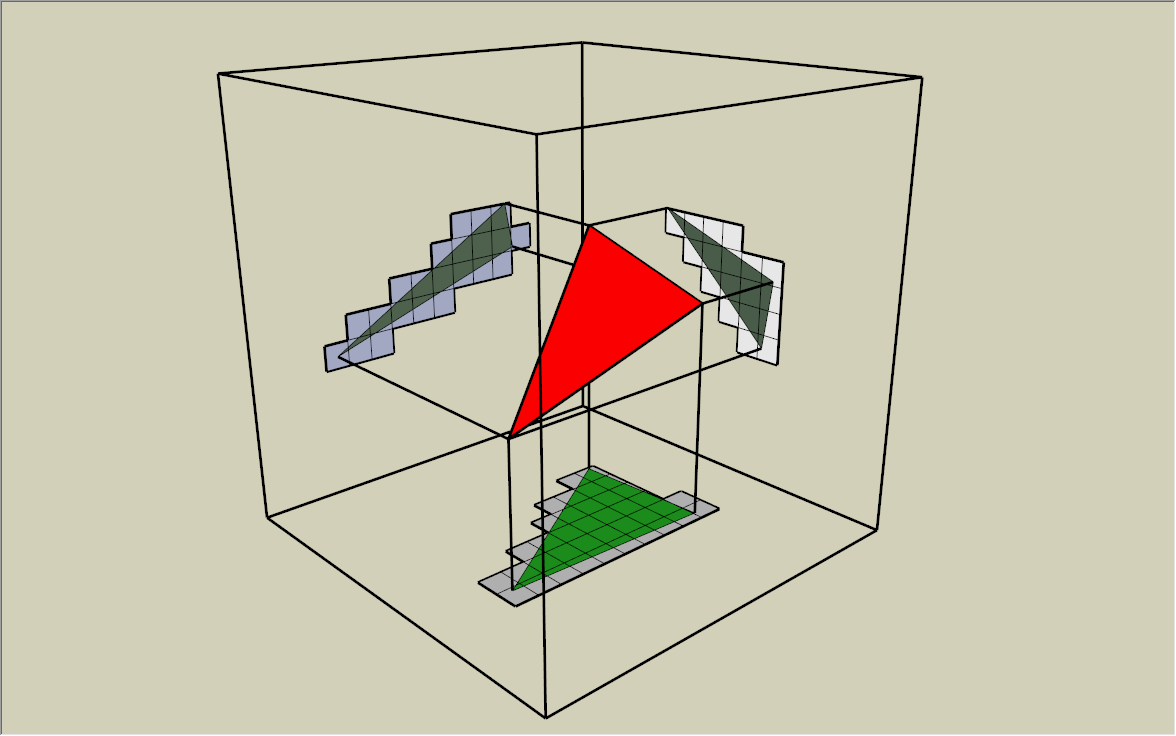
\includegraphics[width=\linewidth]{media/Voxelization_blog_fig_5.png}
		\caption*{Tres direcciones potenciales de proyección.}
	\end{subfigure}%
	\hspace{0.01\textwidth}
	\begin{subfigure}[t]{.49\linewidth}
		\centering
		\captionsetup{justification=centering}
		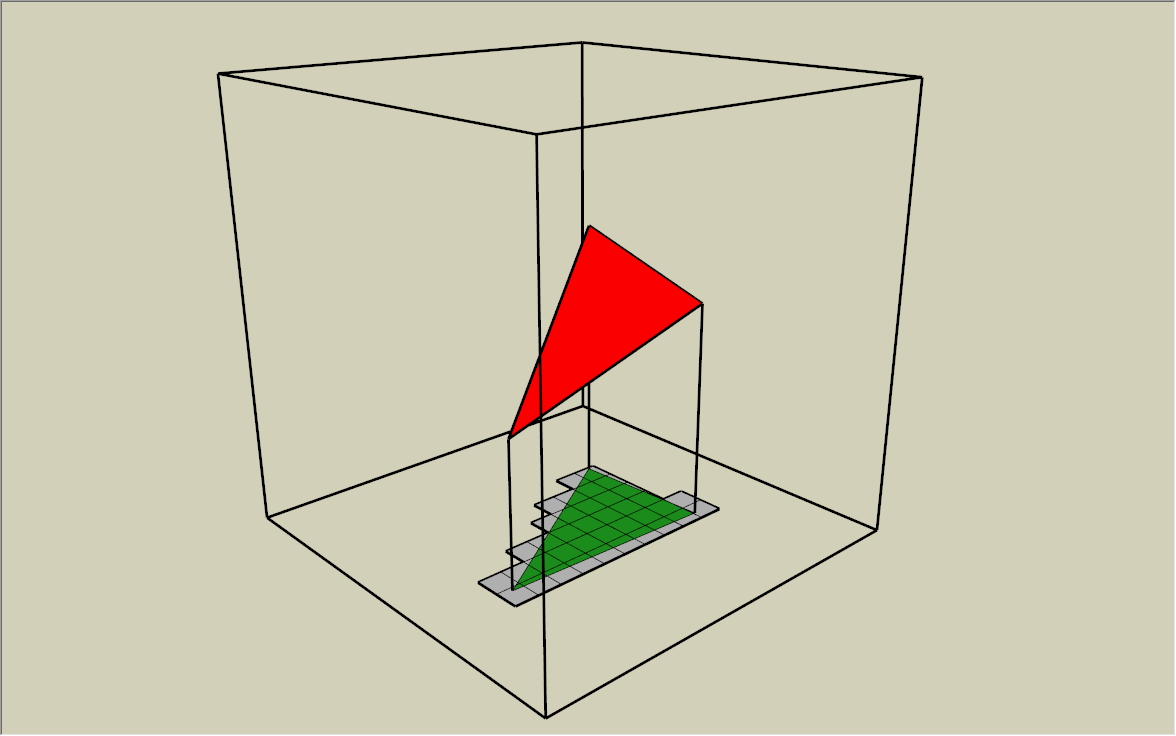
\includegraphics[width=\linewidth]{media/Voxelization_blog_fig_6.png}
		\caption*{Según la normal, proyección al eje Y es lo indicado.}
	\end{subfigure}%
	\caption{Descripción grafica del proceso de selección del eje de proyección. Fuente: Masaya Takeshige, \emph{The Basics of GPU Voxelization} \cite{gpuvoxelization}.}
	\label{fig:axis_selection}
\end{figure}

\subsubsection{Extensión del Triángulo y Polígono Delimitante}
Una vez proyectados todos los vértices del triángulo según el eje direccional escogido (esto es multiplicar cada vértice por la matriz de proyección) entonces se procede a expandir los vértices de este triángulo. Antes de esto primero es importante definir un \ac{AABB} para el triángulo. Este volumen delimitante es utilizado en el fragment shader para descartar fragmentos excedentes del triángulo expandido. El punto mínimo y máximo se expanden según la longitud diagonal de un pixel, en nuestra implementación este valor es $\frac{1}{V_{res}}$ donde $V_{res}$ representa la resolución del volumen.
\\
\begin{lstlisting}[caption={Creacion de un \ac{AABB} para el triángulo proyectado.}, label=AxisAlignedBoundingBox]
vec4 AxisAlignedBoundingBox(vec4 pos[3], vec2 pixelDiagonal)
{
	vec4 aabb;

	aabb.xy = min(pos[2].xy, min(pos[1].xy, pos[0].xy));
	aabb.zw = max(pos[2].xy, max(pos[1].xy, pos[0].xy));

	// enlarge by half-pixel
	aabb.xy -= pixelDiagonal;
	aabb.zw += pixelDiagonal;

	return aabb;
}
\end{lstlisting}

Primero se calculan los planos formados por cada par de vértices del triángulo, perpendiculares al triangulo. Estos planos son trasladados medio pixel hacia afuera con respecto triangulo proyectado.
\\
\begin{lstlisting}[caption={Planos por cada par de vértices del triángulo proyectado.}, label=TPlanes]
vec2 halfPixel = vec2(1.0f / volumeDimension);
// calculate the plane through each edge of the triangle
// in normal form for dilatation of the triangle
vec3 planes[3];
planes[0] = cross(pos[0].xyw - pos[2].xyw, pos[2].xyw);
planes[1] = cross(pos[1].xyw - pos[0].xyw, pos[0].xyw);
planes[2] = cross(pos[2].xyw - pos[1].xyw, pos[1].xyw);
planes[0].z -= dot(halfPixel, abs(planes[0].xy));
planes[1].z -= dot(halfPixel, abs(planes[1].xy));
planes[2].z -= dot(halfPixel, abs(planes[2].xy));
\end{lstlisting}

Luego se calcula la intersección entre los planos perpendiculares al triangulo.
\\
\begin{lstlisting}[caption={Intersección entre planos perpendiculares al triangulo proyectado.}, label=TPlanes2]
// calculate intersection between translated planes
vec3 intersection[3];
intersection[0] = cross(planes[0], planes[1]);
intersection[1] = cross(planes[1], planes[2]);
intersection[2] = cross(planes[2], planes[0]);
intersection[0] /= intersection[0].z;
intersection[1] /= intersection[1].z;
intersection[2] /= intersection[2].z;
\end{lstlisting}

Finalmente se obtienen los vértices del triángulo expandido.
\\
\begin{lstlisting}[caption={Vértices del triángulo expandido.}, label=TPlanes3]
vec4 trianglePlane;
trianglePlane.xyz = cross(pos[1].xyz - pos[0].xyz, pos[2].xyz - pos[0].xyz);
trianglePlane.xyz = normalize(trianglePlane.xyz);
trianglePlane.w = -dot(pos[0].xyz, trianglePlane.xyz);
// calculate dilated triangle vertices
float z[3];
z[0] = -(intersection[0].x * trianglePlane.x + intersection[0].y * trianglePlane.y + trianglePlane.w) / trianglePlane.z;
z[1] = -(intersection[1].x * trianglePlane.x + intersection[1].y * trianglePlane.y + trianglePlane.w) / trianglePlane.z;
z[2] = -(intersection[2].x * trianglePlane.x + intersection[2].y * trianglePlane.y + trianglePlane.w) / trianglePlane.z;
pos[0].xyz = vec3(intersection[0].xy, z[0]);
pos[1].xyz = vec3(intersection[1].xy, z[1]);
pos[2].xyz = vec3(intersection[2].xy, z[2]);
\end{lstlisting}

Este nuevo triangulo expandido es enviado al pipeline de rasterización donde cada fragmento generado será procesado por el fragment shader. En el fragment shader se almacenara los datos de la escena sobre el volumen de vóxeles.

\subsubsection{Composición de Fragmentos y Vóxeles}

% Cada vez que se revoxeliza la escena los volúmenes utilizados durante el proceso de voxelización deben ser limpiados antes de usarse. Para la voxelización estática esto es sencillo, OpenGL provee una función llamada \emph{glClearImage} desde la versión 4.4 la cual permite llenar una textura con un valor indicado a esta función. Debido a que utilizamos el mismo volumen para la voxelización estática no podemos utilizar esta función durante la voxelización dinámica ya que se eliminarían todos los vóxeles estáticos.

% section pipeline_de_voxelizacion (end)
